\documentclass{article}
\usepackage[utf8]{inputenc}
\usepackage{graphicx}

\begin{document}
\title{Relatório Técnico 1}
\author{Rodrigo R. G. e Souza}
\maketitle

O desenvolvimento de software é uma atividade complexa, etc. e tal. Dijkstra disse que para lidar com essa complexidade deve-se decompor os problemas em problemas menores, refinamentos sucessivos. Desde então esse mecanismo de abstração foi incorporado nas linguagens de programação, com o advento da programação estruturada, seguida pela programação orientada a objetos e, mais recentemente, a programação orientada a aspectos. Essa decomposição certamente é útil para diminuir a complexidade do desenvolvimento de software, uma vez que permite dividir a tarefa de desenvolvimento em pedaços intelectualmente assimiláveis, mas faz emergir uma complexa rede de interações entre esses componentes.

Uma forma de entender um sistema é olhando a estrutura de relacionamentos entre seus componentes. Essa análise permite avaliar se o sistema é fácil de modificar, de reusar // Essa estrutura é responsável por tornar um sistema mais fácil ou mais difícil de modificar ou de reusar.
Compreender a maneira como os componentes são interconectados é de grande importância para entender os internos de um software e tirar conclusões sobre seu desenvolvimento. Dois componentes que não interagem entre si podem ser desenvolvidos por duas equipes trabalhando independentemente, sem necessidade de comunicação entre membros de equipes distintas: o funcionamento de um componente não depende do bom funcionamento do outro. Se, no entanto, um componente A precisa de um componente B para funcionar corretamente, um mau funcionamento de B pode causar falhas no componente A.

Essa rede de relacionamentos é usada em análise de impacto de mudanças em software, na divisão de trabalho entre equipes. Curiosamente redes de software de larga escala exibem padrões marcantes, que parecem não depender da linguagem de programação ou da metodologia usada durante o desenvolvimento.

Vamos entender de que forma um programa orientado a objetos é estruturado, as formas como os componentes  interagem entre si e como essas interações podem ser extraídas a partir do código-fonte do programa. A partir daí mostraremos que passos já foram dados na determinação de um modelo da rede de dependências de software.

\section{Redes de Dependências entre Componentes}

Todo programa é dividido em componentes que se relacionam a fim de resolver um problema. Componente, neste caso, é um conceito cujo significado concreto depende do paradigma de programação. Na programação estruturada, os componentes são os procedimentos e as funções; na programação orientada a objetos, são classes (que, por sua vez, são decompostas em componentes chamados métodos e atributos). Neste texto nos concentraremos no caso da programação orientada a objetos.

As formas de interação entre componentes podem ser classificadas em dois tipos: transferência de controle e transferência de dados. A transferência de controle ocorre, por exemplo, quando um método em execução chama um método de outra classe, efetivamente causando a execução do outro método. A transferência de dados pode ocorrer quando parâmetros estão associados a uma chamada de método, ou quando dois objetos compartilham um arquivo.

Essa rede de relacionamentos pode ser modelada por um grafo orientado rotulado, onde os vértices representam os componentes e os arcos representam as interações entre os componentes. O rótulo de um vértice indica o tipo de componente que ele representa (classe, método ou atributo); o rótulo de um arco representa o tipo de relacionamento entre componentes (chamada de método, leitura de atributo, entre outros).

Dizemos que um componente depende de outro quando o primeiro componente requer a presença do segundo para funcionar.

A rede de dependências entre componentes de um programa pode ser extraída automaticamente por um programa construído para este fim, denominado extrator. As técnicas mais comuns de extração de dependências são a análise dinâmica e a análise estática. A análise dinâmica consiste em instrumentar o programa sob análise e então coletar dados sobre sua execução. Esse tipo de análise exige que o programa esteja corretamente instalado e configurado e depende da execução de diversos cenários de uso.

Análise estática é qualquer análise que não depende da execução do programa analisado. As interações entre os componentes são extraídas a partir do código-fonte ou do código objeto do programa analisado. A tabela XXX mostra os tipos de dependência que podem ser extraídos através de análise sintática (cite XXX).

Os dois tipos de análise diferem quanto ao conjunto de relacionamentos que são capazes de extrair de um programa, e mesmo duas técnicas de um mesmo tipo podem fornecer conjuntos distintos. Um estudo comparativo entre extratores pode ser encontrado em XXX. 

Em qualquer caso é impossível garantir que todas as dependências foram extraídas. O problema de determinar se existe uma relação de dependência entre dois componentes é indecidível \cite{Landi1992}. Basta considerar o uso de ponteiros em linguagens como C++, ou a transferências de dados através de arquivos. Assim, o resultado de qualquer ferramenta de análise de dependências deve ser considerado apenas uma aproximação da realidade.

// A Figura 1 mostra uma rede.
// A Figura 2 mostra uma rede simplificada.

// Redes orientadas, não orientadas, colaboração entre classes, filtragem, lifting, abstracting...

Uma rede de dependências entre componentes contém muita informação e pode precisar ser simplificada para análise. Para este fim são empregadas duas técnicas: filtragem e abstração. Filtragem consiste em remover elementos da rede. Por exemplo, Myers considerou em sua análise apenas os relacionamentos de agregação e herança. Mancoridis sugere remover da análise os vértices com grau de entrada muito alto. Abstração consiste em agrupar vértices e os respectivos arcos. É comum representar uma classe, seus métodos e atributos em apenas um vértice. Assim a rede se reduz a uma rede de dependências entre classes, abstraindo detalhes sobre métodos e atributos.

Também acontece de se considerar uma versão não-orientada da rede, onde o sentido (direção) da dependência é desprezado.

// CDN: rede de dependências entre componentes.
Alguns usam direcionado, outros não, alguns usam apenas agregação, alguns usam peso, alguns descartam componentes de bibliotecas, etc.


Outra forma de abstração envolve o emprego de algoritmos de agrupamento (clustering) como o k-means ou o algoritmo hierárquico aglomerativo.

    Além disso, características inerentes a sistemas orientados a objetos, como o polimorfismo, a ligação dinâmica, a herança e o encapsulamento contribuem diretamente para tornar a tarefa da análise de impacto ainda mais dispendiosa. O polimorfismo e a ligação dinâmica permitem que objetos diferentes sejam usados através de suas interfaces, o que será definido somente em tempo de execução. Com o encapsulamento, os objetos ocultam suas implementações, restringindo a forma de observá-los; apenas seus métodos públicos são visíveis. Já com a herança, uma mudança na superclasse pode ou não afetar a subclasse, o que complica a tarefa de analisar o impacto quando uma superclasse é modificada.

// Tipos de dependências: página 29 da diss. de Lile.

Entidades: método, classe, ...
Tipos de relacionamento: chama, estende, lê, altera, agrega, herda...
Significado da dependência (importância na engenharia de software): não dá pra usar um sem o outro, o funcionamento correto de um é necessário para o funcionamento correto de outro, propagação de bugs, distribuição independente, desenvolvimento independente (ver anotação no meu gmail)...
Lifting para o nível de classes

\section{Redes Complexas}

A teoria das redes complexas estuda propriedades gerais de diversos tipos de redes com o uso de ferramentas estatísticas. Estudos realizados na última década revelaram similaridades entre diversas redes, sejam elas tecnológicas, como a Web e a rede de distribuição de energia elétrica dos Estados Unidos, biológicas, como a cadeia alimentar de XXX e ligações entre proteínas da bactéria XXX, ou sociais, como as relações de amizade entre alunos de uma escola.

\subsection{Caracterização de Redes Complexas}

Em 1999, Barabási e Albert \cite{Barabasi1999} analisaram uma amostra da $World Wide Web$, modelada como um grafo não-orientado no qual os vértices representam páginas e as arestas representam links entre duas páginas. Ao agrupar os vértices de acordo com seu grau (número arestas ligadas ao vértice) e plotar o gráfico da frequência de vértices por grau, eles encontraram uma curva que podia ser aproximada por uma lei de potência: a probabilidade de um vértice escolhido ao acaso possuir grau $k$, $P(k)$, é tal que $P(k) \sim k^{-\gamma}$. Essa função é dita livre de escala, pois $P(ak) = bP(k)$ --- a mudança de escala da variável dependente não altera a variável independente a menos de um fator multiplicativo. Desde então foram encontradas distribuições de graus livres de escala em redes biológicas, sociais e tecnológicas, incluindo redes de dependências entre componentes de programas de computador \cite{Valverde2003}.

\begin{figure}
\centering
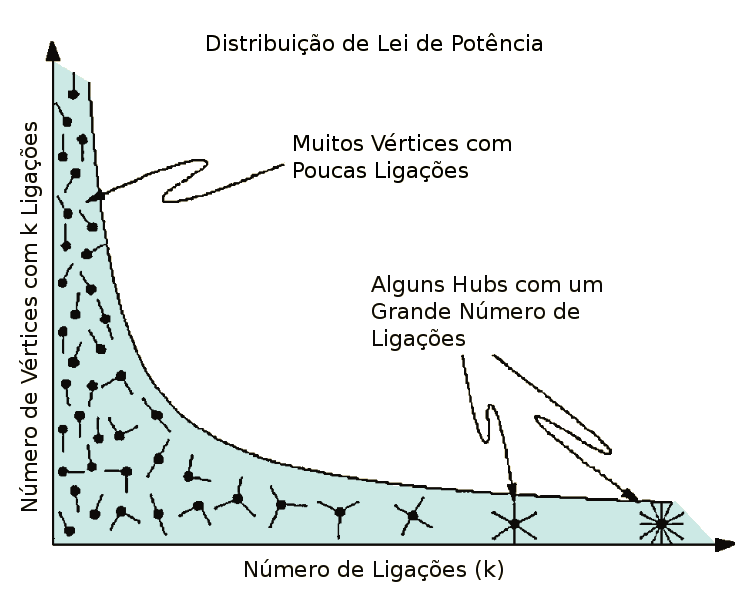
\includegraphics[width=0.5\textwidth]{leidepotencia}
\caption{Lei de potência. Adaptado de \cite{Barabasi2007}}
\end{figure}


Esse resultado foi considerado surpreendente, pois contradiz a hipótese de que redes reais obedecem ao modelo de Erdős-Rényi \cite{Erdos1959}, também chamado de modelo de rede aleatória. Nesse modelo, a probabilidade de um par de vértices ser ligado por uma aresta é constante e igual a $p$ e demonstra-se que a distribuição dos graus é bem aproximada pela distribuição de Poisson.

Uma característica das redes livres de escala é a presença de vértices cujo grau é muito maior do que a média (informalmente chamados de \textit{hubs}). No caso de redes de Erdős-Rényi a probabilidade de existir um vértice com um determinado grau $k$ cai exponencialmente à medida que $k$ se afasta do valor médio e, por essa razão, nessas redes os \textit{hubs} são altamente improváveis.

Barabási e Albert propuseram um modelo para explicar a formação das redes com distribuição de graus livre de escala, formado por dois mecanismos: crescimento contínuo e ligação preferencial \cite{Albert2002}. O modelo propõe que as redes crescem um vértice por vez e cada novo vértice se liga a um número fixo de vértices antigos, dando preferência aos vértices com maior grau (mais formalmente, a probabilidade de um vértice receber uma aresta é proporcional ao seu grau). Hoje sabe-se que redes livres de escala podem ser geradas por diversos modeos \cite{Albert2000,Kumar2000,Aiello2000b,Dorogovtsev2002,Bollobas2003,Deo2005}.

Além da distribuição de graus, muitas redes complexas têm sido caracterizadas pelo efeito mundo pequeno, pelo alto coeficiente de agrupamento e pela presença de motivos.

% Cada vértice em um grafo é caracterizado por um grau, k, que representa a quantidade de arestas ligadas a ele. No caso de grafos orientados, existe a distinção entre grau de saída e grau de entrada, que representam a quantidade de arcos que saem ou entram, respectivamente, do vértice.

\subsubsection{Efeito Mundo Pequeno}

A distância entre dois vértices de uma rede é o número de arestas do menor caminho que conecta os vértices. Diz-se que uma rede apresenta o efeito mundo pequeno quando a distância entre dois vértices é, em média, pequena, mesmo quando a rede é grande. Mais formalmente, a distância média entre vértices é proporcional ao logaritmo do número de vértices. O modelo de Watts e Strogatz \cite{Watts1998}, também conhecido como modelo de mundo pequeno, foi o primeiro modelo a apresentar esse efeito.

%Demonstra-se que tanto os grafos gerados pelo modelo de Erdős-Rényi quanto aqueles gerados pelo modelo de Barabási-Albert possuem essa propriedade.

% Nesse modelo os vértices são dispostos em uma circunferência e então cada vértice se conecta a um número fixo de vértices mais próximos. O grafo resultante é regular, isto é, todos os seus vértices possuem o mesmo grau. A seguir são criadas arestas entre pares de vértices escolhidos aleatoriamente. Essas arestas criam atalhos na rede e fazem com que a rede tenha a propriedade de mundo pequeno. // Rewire

\subsubsection{Coeficiente de agrupamento}


// Em muitas redes, se um vértice A está conectado a dois vértices, B e C, é muito provável que exista uma aresta entre B e C.

Os vizinhos de um vértice são todos os vértices com os quais ele compartilham uma aresta. O coeficiente de agrupamento de um vértice, $C_i$, é a fração de todos os possíveis pares de vizinhos do vértice que estão ligados por uma aresta, e é dado pela seguinte expressão:

\[  C_i = \frac{2x}{k_i(k_i - 1)} \]

onde $x$ é o número de pares de vizinhos do vértice $i$ que estão ligados por uma aresta e $k_i$ é o grau do vértice $i$ \cite{Watts1998}. Por definição, $C_i = 0$ quando $k_i < 2$. Define-se o coeficiente de agrupamento de um grafo, C, como a média aritmética dos coeficientes de agrupamento dos seus vértices. Demonstra-se que o coeficiente de agrupamento de uma rede aleatória de Erdős-Rényi é igual a $\langle k \rangle / n$ (onde $\langle k \rangle$ é o grau médio). Muitas redes complexas possuem um coeficiente de agrupamento alto, isto é, muito maior do que o coeficiente das redes aleatórias.

Outra característica observada em algumas redes é que o coeficiente de agrupamento de um vértice é inversamente proporcional ao grau do vértice, ou seja, $C(k) \sim k^-1$. Segundo Ravasz e Barabási \cite{Ravasz2003}, isso indica a presença de organização hierárquica na rede.

<wiki:comment>
	\cite{Valverde2005,Ma2008}
	

	Motifs ainda é uma linha de pesquisa que precisa amadurecer e, por isso, vai ficar de fora deste relatório

	== Motivos ==

	Global vs. local

	Motifs,
	introduced in [1] are small sub-networks or patterns of
	vertices and edges which occur with in the network. A
	motif is considered to be interesting if it occurs unusually
	frequently in the network.

	Patterns of interconnections occurring in
	complex networks (small-world/scale-
	free) at numbers that are significantly
	higher than those in randomized
	networks.

	network motifs: recurring, significant patterns of interconnections \cite{Milo2002}.

</wiki:comment>

\section{Redes de Dependências entre Componentes como Redes Complexas}

Estudos recentes têm aplicado a teoria das redes complexas em redes de dependências entre componentes de \textit{software}. Valverde e Solé \cite{Valverde2003} detectaram distribuições de graus livres de escala e alto coeficiente de agrupamento em redes não-orientadas formadas por relações de agregação de tipos em diagramas UML, programas em C e programas em C++. Myers \cite{Myers2003} analisou redes de chamadas de função em programas em C e redes de agregação e herança em programas em C++, modeladas como grafos orientados. Em ambos os casos ele identificou organização hierárquica através da distribuição do coeficiente de agrupamento, $C(k) \sim k^{-1}$. O estudo revelou uma correlação negativa entre o grau de entrada e o grau de saída de um vértice. Leis de potência foram encontradas tanto na distribuição de graus de entrada quanto na distribuição dos graus de saída.

Distribuições de graus livres de escala também foram encontradas encontradas em programas escritos em Smalltalk \cite{Marchesi2004,Concas2007}, em Java \cite{Hyland-Wood2006,Baxter2006,Ichii2008}, em dependências entre pacotes de \textit{software} \cite{Labelle2004}, em chamadas de sistema, em dependências entre bibliotecas dinâmicas \cite{Louridas2008} e até mesmo em referências entre objetos em tempo de execução \cite{Potanin2005}.

É difícil comparar as pesquisas porque nem sempre elas deixam explícito quais tipos de relacionamento entre componentes foram considerados para a construção das redes. Alguns trabalhos usam ferramentas estatísticas inadequadas para leis de potência (veja a seção \ref{sec:estatistica}).

%Nem todos os trabalhos usam a Estatística rigorosamente. Lognormal, double pareto, power law, stretched exponential, power law with exponential cutoff... Alguns usam o coeeficiente de determinação ($R^2$), que não se aplica a leis de potência, ou o método dos mínimos quadrados sobre o logaritmo dos dados.

\section{Apêndice: Tratamento Estatístico de Leis de Potência} \label{sec:estatistica}

// Talvez aqui fazer algo didático, como no livro The Black Swan

Propriedades estatísticas da lei de potência. A Figura 1(a) mostra o gráfico de uma lei de potência. Intuitivamente, percebe-se que a grande maioria dos vértices possui um grau pequeno, mas existem vértices cujo grau está muito acima do grau médio. Trata-se de uma curva assimétrica positiva, pois a média é maior do que a mediana. A probabilidade de um elemento de grau alto é pequena mas não desprezível, e isso contribui para elevar a média. Como a distribuição é muito heterogênea, a média não é um valor muito representantivo da distribuição. A lei de potência, quando plotada em escala log-log, se apresenta sob a forma de uma reta. Dificilmente dados obtidos experimentalmente formam uma reta em toda sua extensão. Portanto muitas vezes quando se afirma que uma distribuição é livre de escala, o que se quer dizer é que parte da distribuição é bem aproximada por uma reta na escala log-log.

Tratamento estatístico de leis de potência:  \cite{Newman2005} - Power laws, Pareto distributions and Zipf's law   //   Clauset et al - Power-law distributions in empirical data \cite{Clauset2007}

histograma. problema com a escolha do tamanho do bin. histograma com exponential bins
distribuição cumulativa complementar (survival)
maximum likelihood estimation para estimar expoente.
goodness-of-fit para estimar região de scaling.
não usar: regressão linear (método dos mínimos quadrados), coeficiente de determinação ($R^2$)



\section{Recuperação de Arquitetura}

\subsection{Arquitetura: Componentes e Conectores}

Componentes e conectores.
Visões. Processos, módulos.

\subsection{Técnicas de Recuperação de Arquitetura}


Análise dinâmica, análise estática. Padrões de nomes (Anquetil). Padrões estrutrais (LIMBO). Análise de clustering (Maqbool)



Sobre clustering. Referência: Introduction to Data Mining, capítulo 8

\subsubsection{Detecção de Comunidades}

= análise de clustering (graph clustering, network clustering), = recuperação de arquitetura modular (módulos de atribuição de trabalho).

Clauset, Newman, Moore - Finding community structure in very large networks \cite{Clauset2004}

Gulbahce2008 - "The art of community detection" \cite{Gulbahce2008}: Currently the state of the art is to design an artificial network with the structural properties that one wants to detect (e.g. group strucutre) and then show that the algorithm being tested is able to detect such structures. 

definição de cluster: A number of similar things collected together or lying contiguous; a group;

A community is
a densely connected subset of nodes that is only sparsely
linked to the remaining network. (Gulbahce)

Communities in a citation network might represent
related papers on a single topic;

Community can be considered as a summary of
the whole network thus easy to visualize and
understand.

relação funcional, módulos de funcionalidade


Modelo de Girvan-Newman - Newman - Fast algorithm for detecting community structure in networks \cite{Newman2004b} e, mais antigo, Newman, Girvan - Finding and evaluating community structure in networks \cite{Newman2004a}

Paper: Benchmark for community detection \cite{Lancichinetti2008}


\subsection{Tipos de Decomposições}

Referência: Introduction to Data Mining, capítulo 8 \cite{Tan2005}

Hierárquica vs partitiva.
Exclusive vs overlapping vs fuzzy.
Completa vs. parcial.

\subsection{Algoritmos}

Bunch. LIMBO. MCL etc. (a escolher)

\subsection{Avaliação de Decomposições}

Avaliação não-supervisionada: NED, estabilidade.
Avaliação supervisionada: authoritativeness.

Avaliações relativas (comparar dois algoritmos)

\subsection{Comparação entre Decomposições}

Precision-recall.
MoJo.
EdgeMoJo.
etc.

\bibliographystyle{apalike}
\bibliography{complex-networks,rodrigo-mestrado}

\end{document}
